\chapter[Implementação do Serviço]{Implementação Do Serviço}
\label{ch:servico}
\section{Visão Geral}

Como proposto inicialmente, este trabalho de conclusão de curso visa a implementação de um Serviço que seja capaz de receber uma base de dados e aplicar os modelos de seleção de características, informando então quais são as características mais relevantes ao problema. O sistema foi implementado para a Web e possui uma interface onde o usuário pode, além de realizar a seleção de características, criar seus projetos e executar os modelos aplicados a cada um deles.

\section{Arquitetura do Serviço}

Durante a elaboração da arquitetura do serviço era preciso pensar em uma maneira de criar uma aplicação Web para que facilitasse o seu acesso, além de poder integrar o uso de outras ferramentas já utilizadas durante esse trabalho. Como os modelos já haviam sido implementados utilizando a biblioteca Weka, foi então necessário encontrar um conjunto de ferramentas que se adequasse à ela, e que pudesse desenvolver uma aplicação Web. Levando em consideração essas premissas foram escolhidos as ferramentas Ruby on Rails \cite{ror} e a linguagem JRuby \cite{jruby}. A combinação da linguagem JRuby com a ferramenta Ruby on Rails, permitiria utilizar o poder e agilidade de desenvolvimento Web da ferramenta Ruby on Rails, junto ao uso de bibliotecas implementadas em Java através do JRuby, sendo então uma ótima combinaçao para desenvolver o sistema. Alguns problemas foram encontrados ao tentar realizar a comunicação das ferramentas, como por exemplo as divergências entre a estrutura da documentação do Weka com a sua estrutura de classes, bibliotecas Ruby que não eram compatíveis com JRuby e tratamento de exceções da biblioteca Weka. Todos os problemas foram resolvidos ao longo do desenvolvimento da aplicação.

Após a escolha das técnologias e ferramentas a serem utilizadas, foi então pensado como seria a arquitetura. A arquitetura do serviço foi pensada para que o usuário submetesse um arquivo contendo a base de dados em que ele gostaria que fosse realizado a Seleção de Características, esse processo segue as seguintes fases:

\begin{enumerate}
	\item{Pré Processamento: Onde a base é trabalhada a fim de deixá-la pronta para que um dos modelos de seleção seja aplicado sobre ela. Essa fase consiste em preencher as lacunas e remover as características que não possam ser utilizadas no classificador kNN, como ja utilizado anteriomente no Capítulo \ref{ch:validacao}}
	\item{Executar Base de Dados: Após a base ser pré processada, ela será executada escolhendo um dos métodos escolhidos e citados no Capítulo \ref{ch:modelos}}
	\item{Atualizar Status da Execução: Quando o processo de execução acabar, será realizada a atualização dos dados da execução, tais como as características escolhidas, a acurácia obtida e o tempo gasto para executar a base de dados.}
\end{enumerate}

O Serviço utiliza-se da arquitetura mostrada na Figura 12.

\begin{figure}[h]
	\centering
		\includegraphics[keepaspectratio=true,scale=0.35]{figuras/fig13.eps}
	\caption{Arquitetura do Serviço de Seleção de Características}
	\label{fig:fig13}
\end{figure}

Podemos ver que o sistema age em sua grande maioria no lado servidor, onde ele realiza o Pré Processamento, a Execução da base de dados e a Atualização do Status da Execução. Podemos perceber também o uso de Threads de processamento para que seja possível melhorar o desempenho do sistema, uma vez que o JRuby utiliza de Threads reais em seu processamento \cite{jruby}, fazendo com que o uso de Threads possua um resultado satisfatório.

Tendo essa visão da arquitetura do sistema, foi pensado como seria o relacionamento entre as diversas entidades do serviço. As principais entidades são \textit{User, Project e Execution}. Essas entidades compõem o sistema para que seja possivel melhor organizar o seu funcionamento. 


Na Figura 13 podemos observar o fluxo de funcionamento do serviço que conta com um sistema de \textit{Login}, onde os usuários fornecem suas credenciais, além de poderem se registrar fornecendo um email e uma senha. Após o usuário se registrar no sistema, ele tem acesso a criação de um projeto, ou selecionar um projeto ja existente para que possa executá-lo. No caso da criação de um novo projeto, o usuário deve fornecer um nome, uma descrição e uma base de dados para que seja possível a sua criação, essa base de dados deve respeitar os pré requisitos descritos mais adiante na fase de Pré Processamento.

\begin{figure}[H]
	\centering
		\includegraphics[keepaspectratio=true,scale=0.35]{figuras/fig17.eps}
	\caption{Fluxograma do Serviço}
	\label{fig:fig14}
\end{figure}

Após realizado esse pré processamento e o projeto tendo sido criado, pode-se executa-lo. Ao escolher executar um projeto, será necessário escolher um modelo de seleção de características dentre os modelos estudados nesse trabalho. Ao escolher um dos modelos, o projeto será executado e então as características começarão a ser escolhidas. Esse processo de seleção é feito em paralelo, e após selecionadas as características, serão mostradas as características selecionadas e a acurácia obtida com essas características. As fases do serviço estão melhor explicadas na próxima seção.

\section{Fases do Serviço}
\label{sec:fases}
O serviço implementado segue as fases que estão listadas abaixo. Essas fases corroboram para o funcionamento da aplicação de modo que o seu fluxo de execução, mostrado na Figura 14, seja executado e, a partir disso, selecionar as características que sejam mais preponderantes ao problema de acordo com os métodos de seleção de características, conforme mostrado nos capítulos anteriores.
\subsection{Pré Processamento}
\label{sec:preprocessamento}
A fase de Pré Processamento é de suma importancia ao serviço pois a base de dados é adquirida nessa fase, e ao ser adquirida ela deve ser analisada para que seja possivel constatar a necessidade de algum tipo de pre processamento, tal como a conversão, pois a biblioteca Weka, que é utilizada para trabalhar as bases de dados, funciona apenas com arquivos do formato \textit{Attribute-Relation File Format} (.arff), sendo assim, qualquer base que não esteja nesse formato não será aceita, salvo a exceção do formato \textit{Comma-separated values} (.csv), onde é utilizado um conversor para que seja possível utilizar essa base se ele estiver no formato descrito na Figura 14.

\begin{figure}[H]
	\centering
	\label{fig15}
		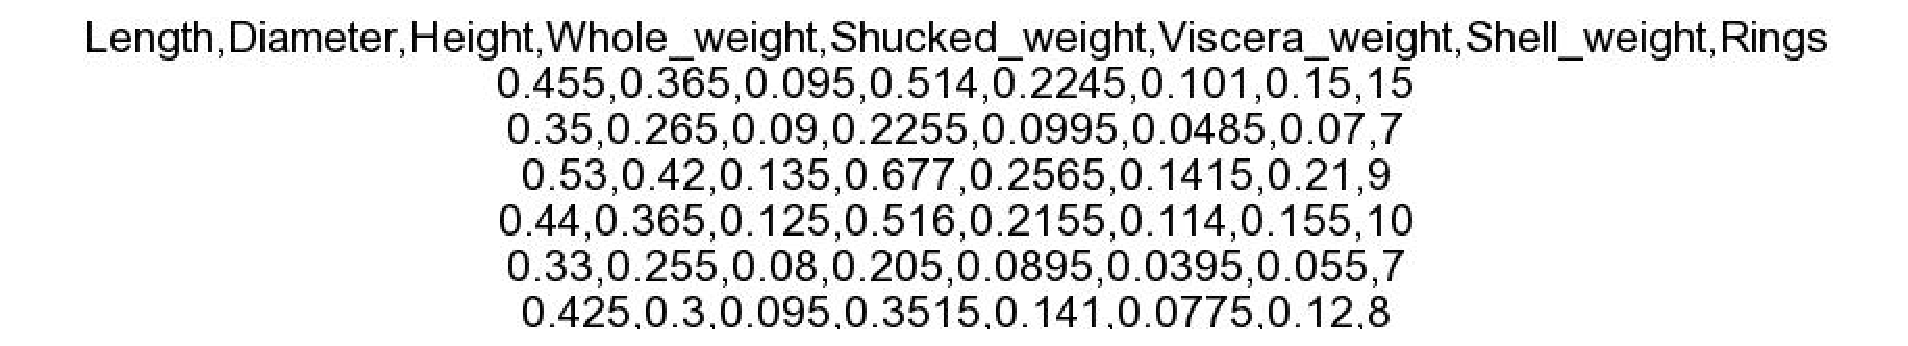
\includegraphics[keepaspectratio=true,scale=0.5]{figuras/fig15.eps}
	\caption{Arquivo Formato .csv}
\end{figure}

Conforme mostrado na figura, a primeira linha deve descrever o nome das características do problema, e as demais linhas devem compor os dados da base, estando cada um dos dados alinhados a sua característica. Percebe-se que todas as informações são separadas por vírgulas, e esse padrão deve ser mantido para que o conversor reconheça a estrutura do arquivo e consiga convertê-lo.

O resultado dessa conversão pode ser observado na Figura 15, onde é possível ver um arquivo .arff já convertido, e como ele é configurado.

\begin{figure}[H]
	\centering
	\label{fig16}
		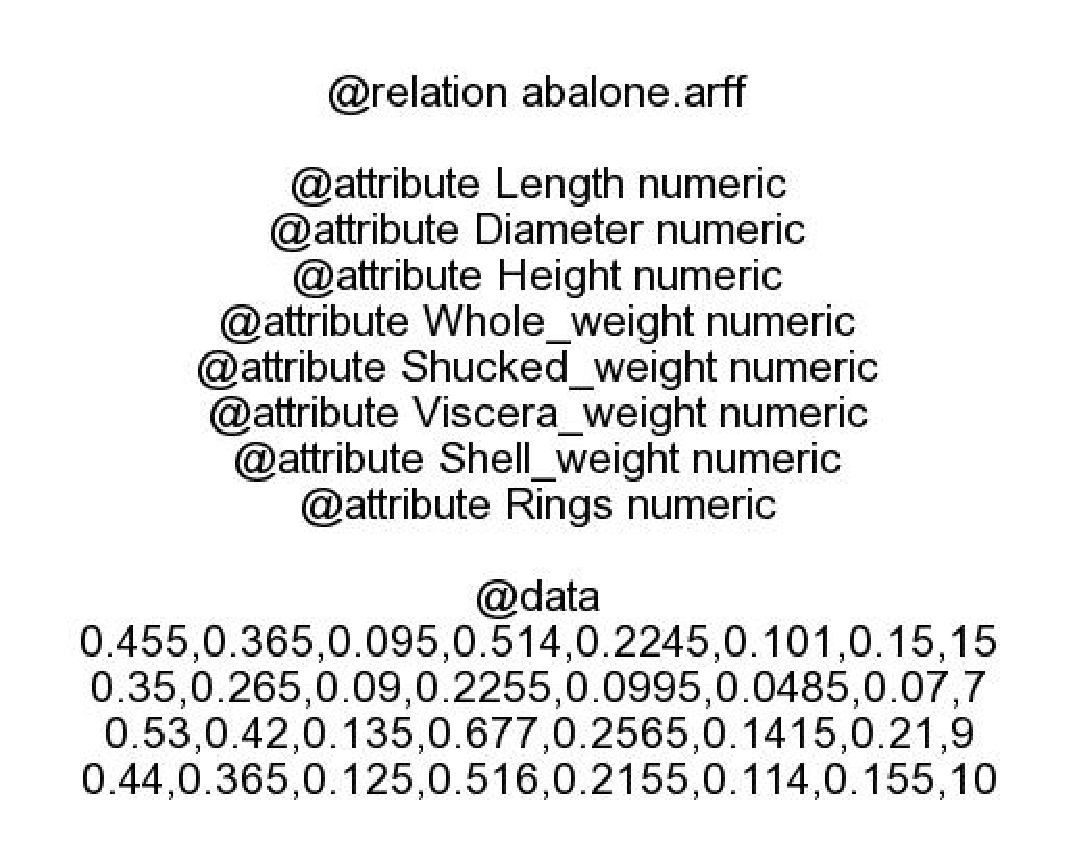
\includegraphics[keepaspectratio=true,scale=0.5]{figuras/fig16.eps}
	\caption{Arquivo Formato .arff}
\end{figure}

Podemos observar que na primeira linha existe o nome da base, depois é descrito cada uma das características e o seu tipo (numérico, nominal, etc. como já dito em capítulos anteriores). Após descrever cada uma das características, é descrito os dados que compõem essa base, seguindo o mesmo padrão que é seguido no .csv, ou seja, separados por virgula.

Além dessa analise da base, também é analisado se existem lacunas na base de dados. Essas lacunas são dados que não estão inclusos, ou seja, estão nulos, e esse tipo de lacuna tende a não ser aceito por alguns classificadores, além de gerar ruído ou atrapalhar o treinamento do modelo \cite{labic_2002}. Para mitigar esse problema o sistema substituirá todas as lacunas pela média, em caso de atributo quantitativo, ou pela moda, em caso de atributo qualitativo. O sistema assume essa abordagem para que se tente evitar o \textit{overfitting}, que é quando um modelo se ajusta aos dados de treinamento e não necessariamente consegue generalizar quando se recebe outros dados \cite{hawkins_2002}.

Após realizadas todas essas etapas, a base finalmente estará pronta para ser executada na fase de Execução da Base de Dados.


\subsection{Execução da Base de Dados}
Durante essa etapa, a base submetida na fase de Pré Processamento será submetida a um dos modelos selecionado pelo usuário, e que foram implementados e mostrados anteriomente neste trabalho, sendo eles: \textit{Relief-F, Decision Tree Method e Linear Forward Selection with kNN}. Quando o usuário seleciona o modelo, e dá inicio a execução da base de dados, o sistema aciona a biblioteca Weka, onde está a implementação dos modelos, e criará uma \textit{Thread} para executa-lo. Quando a \textit{Thread} finaliza o seu processamento, ela irá concluir a execução e passará para a próxima fase.

\subsection{Atualização do Status da Execução}
Após realizado a seleção de características pela fase de Execução da Base de Dados, terá inicio a fase de Atualização do Status da Execução, onde serão atualizados os dados da execução criada, mostrando as características que foram selecionadas após a execução do modelo, a acurácia dessas características aplicadas a um classificador kNN, a acurácia com todas as características, e o tempo gasto para que fosse executado esse método. O usuário poderá então visualizar quais são as características mais preponderantes ao seu modelo, e todos os outros dados citados.